\begin{anexosenv}

\partanexos

\chapter{Caso de uso 001}\label{CASO001}

\section*{Inserção de Dados}

\subsection*{Descrição}
O sistema irá inserir informações referentes a licitações no banco de dados.

\subsection*{Atores}
Sistema.

\subsection*{Pré-condições}
O serviço onde a informação sobre licitação precisa estar disponível.

\subsection*{Fluxo Principal}
\begin{enumerate}
    \item\label{FP001001} O ator buscará as informações na API de acesso a informação compras governamentais~[\regra{rn009}]
    \item O ator tratará as informações colhidas~[\regra{rn010}]
    \item O ator insere as informações no banco de dados~[\regra{rn011}]
\end{enumerate}

\subsection*{Fluxo de Exceção}
\begin{enumerate}
    \item Se no Passo~\ref{FP001001} do Fluxo Principal, o ator buscar essas informações e o serviço estiver indisponível, o sistema preencherá no log que houve falha.
\end{enumerate}

\subsection*{Regras de Negócio}
\subsubsection*{RN001}\label{rn009}
A busca será feita todos os dias a partir de 01:00.
\subsubsection*{RN002}\label{rn010}
As informações que vão ser inseridas é: licitação, item, material e serviço.
\subsubsection*{RN003}\label{rn011}
A inserção será após a regra de negócio~[\regra{rn010}].

\chapter{Caso de uso 002}\label{CASO002}

\section*{Solicitar inclusão}

\subsection*{Descrição}
O sistema deverá permitir ao usuário solicite a inclusão de um item em uma licitação.

\subsection*{Atores}
Servidor público.

\subsection*{Pré-condições}
O Ator deverá estar autenticado e autorizado.

\subsection*{Fluxo Principal}
\begin{enumerate}
    \item Ator aciona o item de menu Home~[\regra{rn002}]
    \item Sistema exibe a tela Home~[\prototipo{PROT001}]
    \item\label{FP002009} Ator seleciona o tipo de item que deseja solicitar clicando em "Material" ou "Serviço"
    \item O sistema exibe as licitações abertas com o item escolhido~[\prototipo{PROT002}]
    \item\label{FP002005} Ator seleciona qual licitação ele deseja solicitar o item e clica em solicitar~[\regra{rn004}]
    \item Sistema exibe tela de descrição da licitação e item selecionado~[\prototipo{PROT003}]
    \item\label{FP002007} Ator escolhe a quantidade de item desejada e clica em solicitar, sistema abre a uma tela auxiliar para confirmar o pedido~[\prototipo{PROT004}]~[\regra{rn003}]
    \item\label{FP002008} O ator clica em ``Sim'' e o sistema redireciona para página inicial informando em uma tela auxiliar o código gerado para a solicitação aberta~[\prototipo{PROT005}].
\end{enumerate}

\subsection*{Fluxo Alternativo}
\begin{enumerate}
    \item Se no Passo~\ref{FP002009},o ator clicar em "Material" o sistema redireciona para página solicitar material~[\prototipo{PROTA001}].
    \item Se no Passo~\ref{FP002009},o ator clicar em "Serviço" o sistema redireciona para página solicitar serviço~[\prototipo{PROTA002}].
    \item Se no Passo~\ref{FP002005}, o ator preencher qualquer um dos filtros e clicar em ``Pesquisar'', retornará a lista de resultados encontrados.~[\regra{rn005}]~[\regra{rn006}]
    \item Se no Passo~\ref{FP002005} do Fluxo Principal, o ator clicar em ``Voltar'', o sistema retorna à tela anterior~[\prototipo{PROT001}]
    \item Se no Passo~\ref{FP002007} do Fluxo Principal, o ator clicar em ``Voltar'', o sistema retorna à tela anterior~[\prototipo{PROT002}]
    \item Se no Passo~\ref{FP002008} do Fluxo Principal, o ator clicar em ``Voltar'', o sistema retorna à tela anterior~[\prototipo{PROT003}]
\end{enumerate}

\subsection*{Fluxo de Exceção}
\begin{enumerate}
    \item Se no Passo~\ref{FP002008} do Fluxo Principal, o ator executa ação diferente das previstas pelos botões na tela, o sistema é redirecionado para uma tela de erro.
\end{enumerate}


\subsection*{Regras de Negócio}

\subsubsection*{RN001}\label{rn002}
O ator deve estar autenticado e autorizado.

\subsubsection*{RN002}\label{rn003}
Campo quantidade deve ser validado

\subsubsection*{RN003}\label{rn004}
Botões selecionar e solicitar devem ser habilitados somente quando as opções forem preenchidas corretamente

\subsection*{Protótipos}
\begin{figure}[htbp]
    \centering
    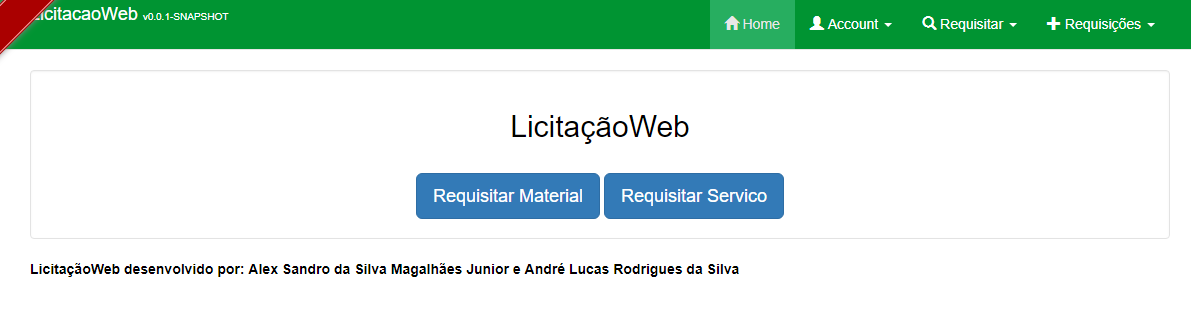
\includegraphics[width=0.95\textwidth]{figuras/prototipo001.png}
    \caption[PROT001: Tela home]{PROT001: Tela home.}
    \label{PROT001}
\end{figure}

\begin{figure}[htbp]
    \centering
    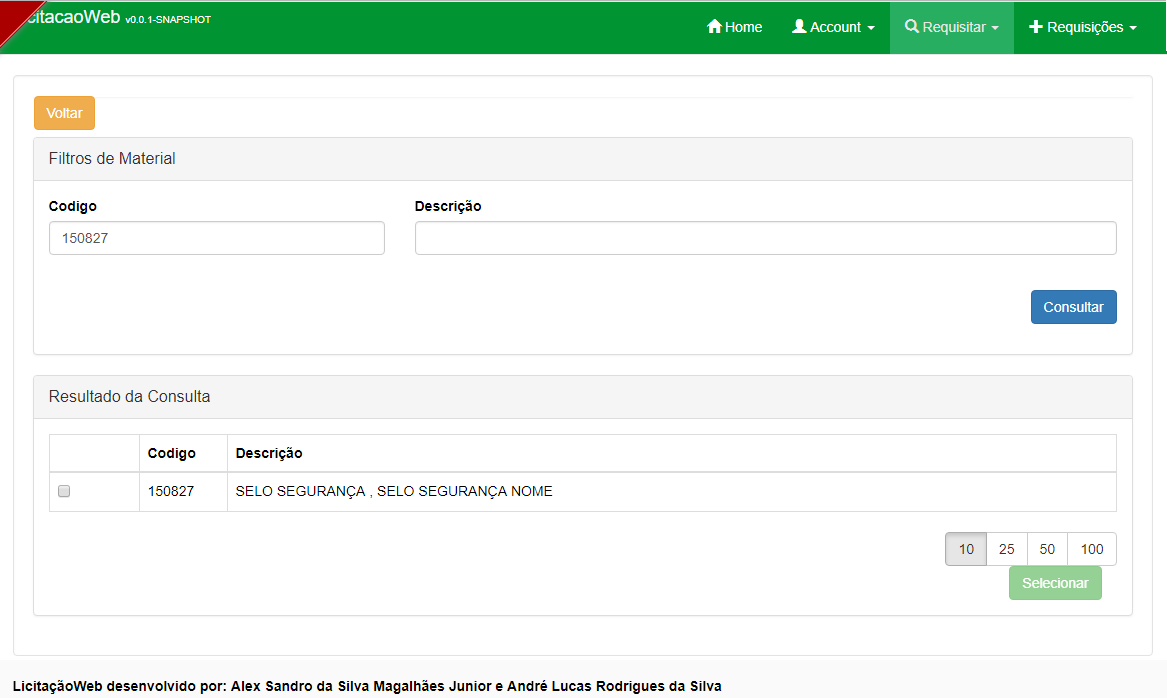
\includegraphics[width=0.95\textwidth]{figuras/prototipoA001.png}
    \caption[PROTA001: Solicitar Material]{PROTA001: Solicitar Material.}
    \label{PROTA001}
\end{figure}

\begin{figure}[htbp]
    \centering   
    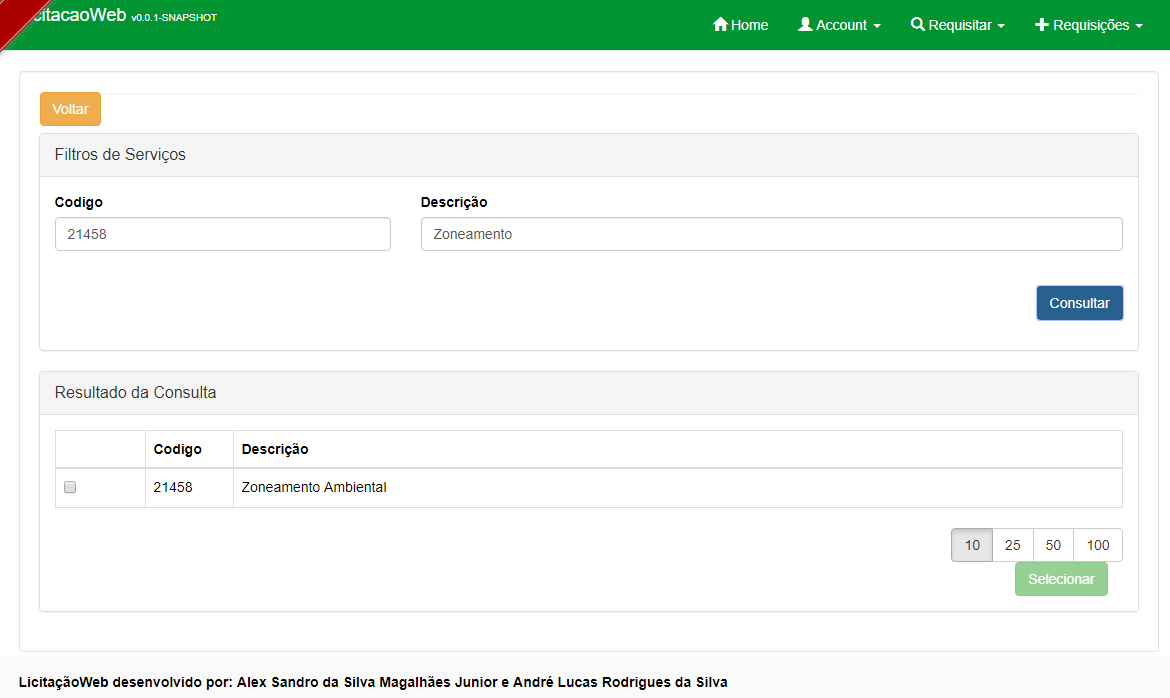
\includegraphics[width=0.95\textwidth]{figuras/prototipoA002.png}
    \caption[PROTA002: Solicitar serviço]{PROTA002: Solicitar serviço.}
    \label{PROTA002}
\end{figure}

\begin{figure}[htbp]
    \centering
    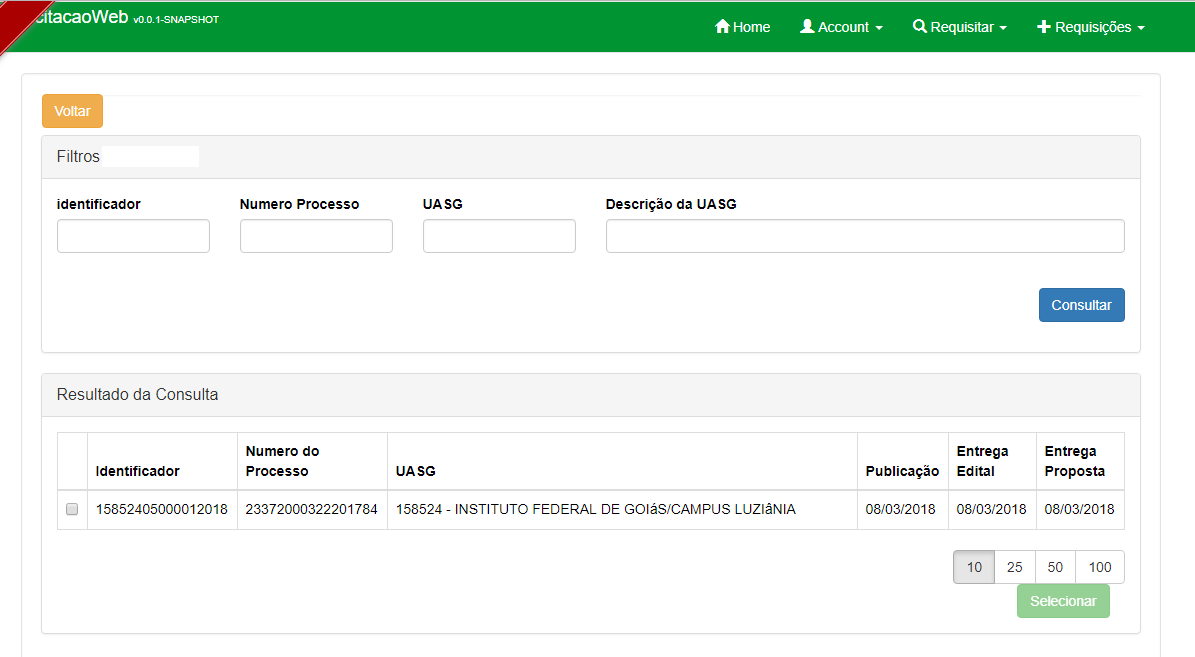
\includegraphics[width=0.95\textwidth]{figuras/prototipo002.png}
    \caption[PROT002: Licitações abertas]{PROT002: Licitações abertas.}
    \label{PROT002}
\end{figure}

\begin{figure}[htbp]
    \centering
    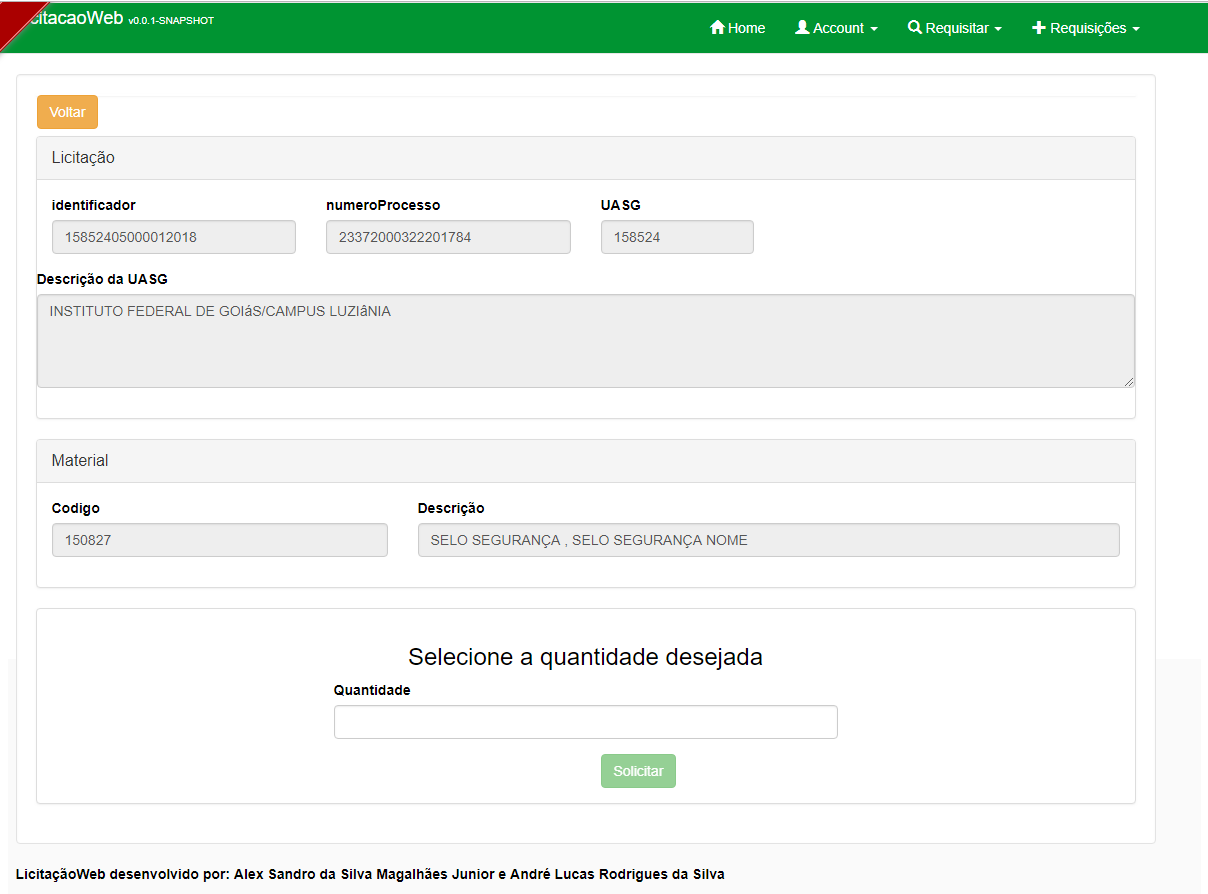
\includegraphics[width=0.95\textwidth]{figuras/prototipo003.png}
    \caption[PROT003: Descrição do item selecionado]{PROT003: Descrição do item selecionado.}
    \label{PROT003}
\end{figure}

\begin{figure}[htbp]
    \centering
    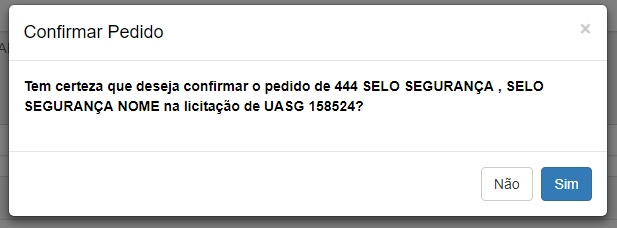
\includegraphics[width=0.95\textwidth]{figuras/prototipo004.png}
    \caption[PROT004: Confirmação de pedido]{PROT004: Confirmação de pedido.}
    \label{PROT004}
\end{figure}

\begin{figure}[htbp]
    \centering
    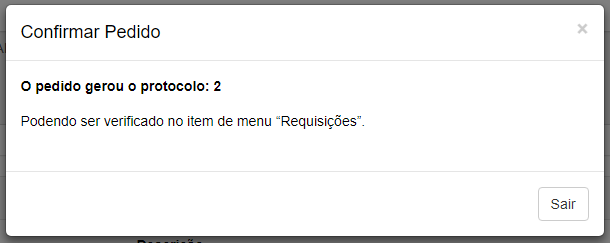
\includegraphics[width=0.95\textwidth]{figuras/prototipo005.png}
    \caption[PROT005: Código gerado do pedido]{PROT005: Código gerado do pedido.}
    \label{PROT005}
\end{figure}

\chapter{Caso de uso 003}\label{CASO003}

\section*{Analisar Requisições}

\subsection*{Descrição}
O sistema permitirá que o usuário analise a solicitação do pedido de participação em uma licitação.

\subsection*{Atores}
Servidor público.

\subsection*{Pré-condições}
O Ator deverá estar autenticado e autorizado.

\subsection*{Fluxo Principal}
\begin{enumerate}
    \item Ator aciona o item de menu ``Requisiçõe''~ e o item do submenu ''Analisar''.[\regra{rn002}].
    \item\label{FP003002} Sistema exibe a tela de Analisar  Requisições~[\prototipo{PROT006}]
    \item\label{FP003003} Ator clica em Analisar, o sistema é redirecionado para a tela de análise~[\regra{rn012}]~[\prototipo{PROT007}].
    \item\label{FP003004} Ator clica em ``Sim'', irá se aberto uma tela de auxílio para confirmar~[\regra{rn007}]~[\prototipo{PROT008}].
    \item\label{FP003005} O ator clica em ``Sim'' e o sistema redireciona para página de Analisar  Requisições~[\prototipo{PROT006}]
\end{enumerate}

\subsection*{Fluxo Alternativo}
\begin{enumerate}
    \item Se no Passo~\ref{FP003002}, o ator preencher qualquer um dos filtros e clicar em ``Pesquisar'', retornará a lista de resultados encontrados.~[\regra{rn005}]~[\regra{rn006}]
    \item Se no Passo~\ref{FP003003} do Fluxo Principal, o ator clicar em ``Voltar'', o sistema retorna à tela anterior~[\prototipo{PROT001}]
    \item Se no Passo~\ref{FP003004} do Fluxo Principal, o ator clicar em ``Não'', o sistema retorna à tela anterior~[\prototipo{PROT006}]~[\regra{rn008}]
    \item Se no Passo~\ref{FP003004} do Fluxo Principal, o ator clicar em ``Cancelar'', o sistema retorna à tela anterior~[\prototipo{PROT006}]
    \item Se no Passo~\ref{FP003005} do Fluxo Principal, o ator clicar em ``Voltar'', o sistema retorna à tela anterior~[\prototipo{PROT007}]
\end{enumerate}

\subsection*{Regras de Negócio}

\subsubsection*{RN001}\label{rn005}
O campo deve ser preenchido com no mínimo 3 caracteres.
\subsubsection*{RN002}\label{rn006}
Botão pesquisar devem se habilitado somente quando as opções forem preenchidas corretamente de acordo com a regra de negócio~[\regra{rn005}]. 
\subsubsection*{RN003}\label{rn007}
Quando o ator confirmar a análise, ira se retornado a resposta para o campus pedinte.
\subsubsection*{RN004}\label{rn008}
Quando o ator negar a análise, ira se retornado a resposta para o campus pedinte.
\subsubsection*{RN005}\label{rn012}
O botão "Analisar" deve ser habilitado quando a situação estiver como “Analise Pendente”.

\subsection*{Protótipos}
\begin{figure}[htbp]
    \centering
    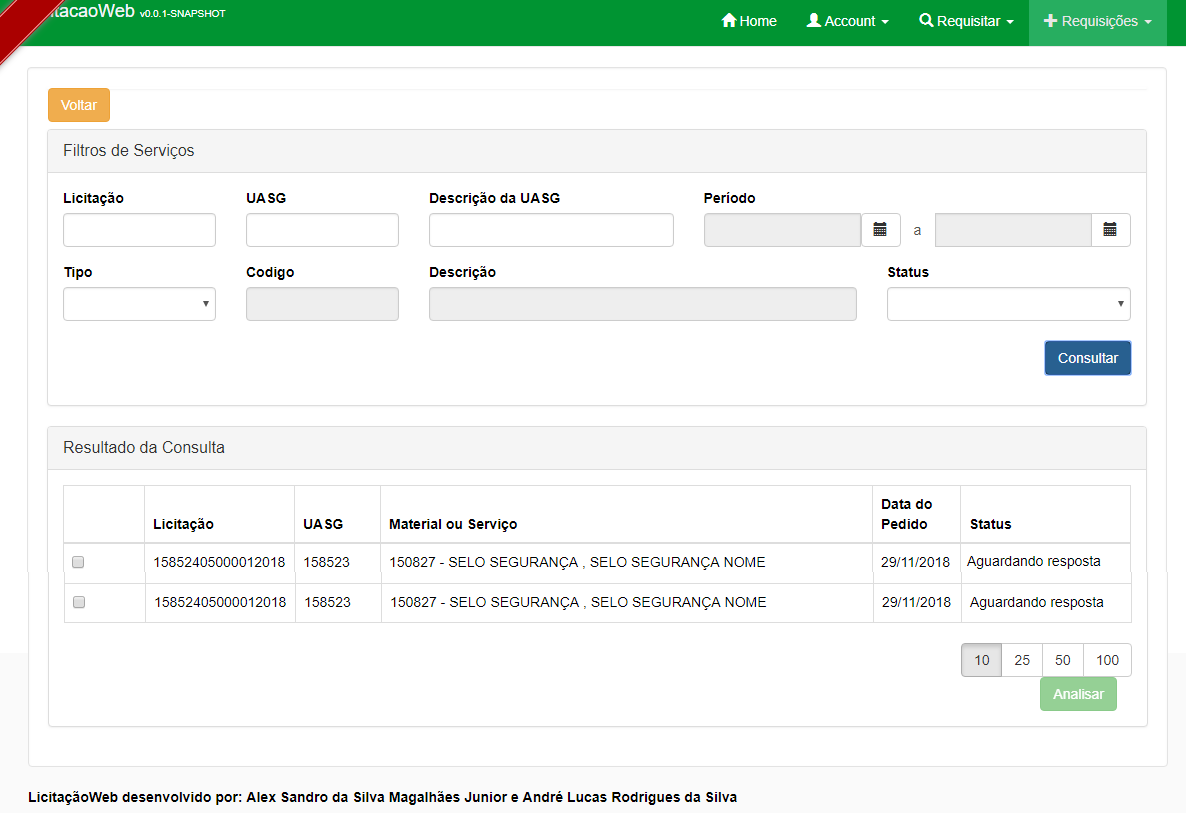
\includegraphics[width=0.95\textwidth]{figuras/prototipo006.png}
    \caption[PROT006: Lista de Requisições]{PROT006: Lista de Requisições.}
    \label{PROT006}
\end{figure}

\begin{figure}[htbp]
    \centering
    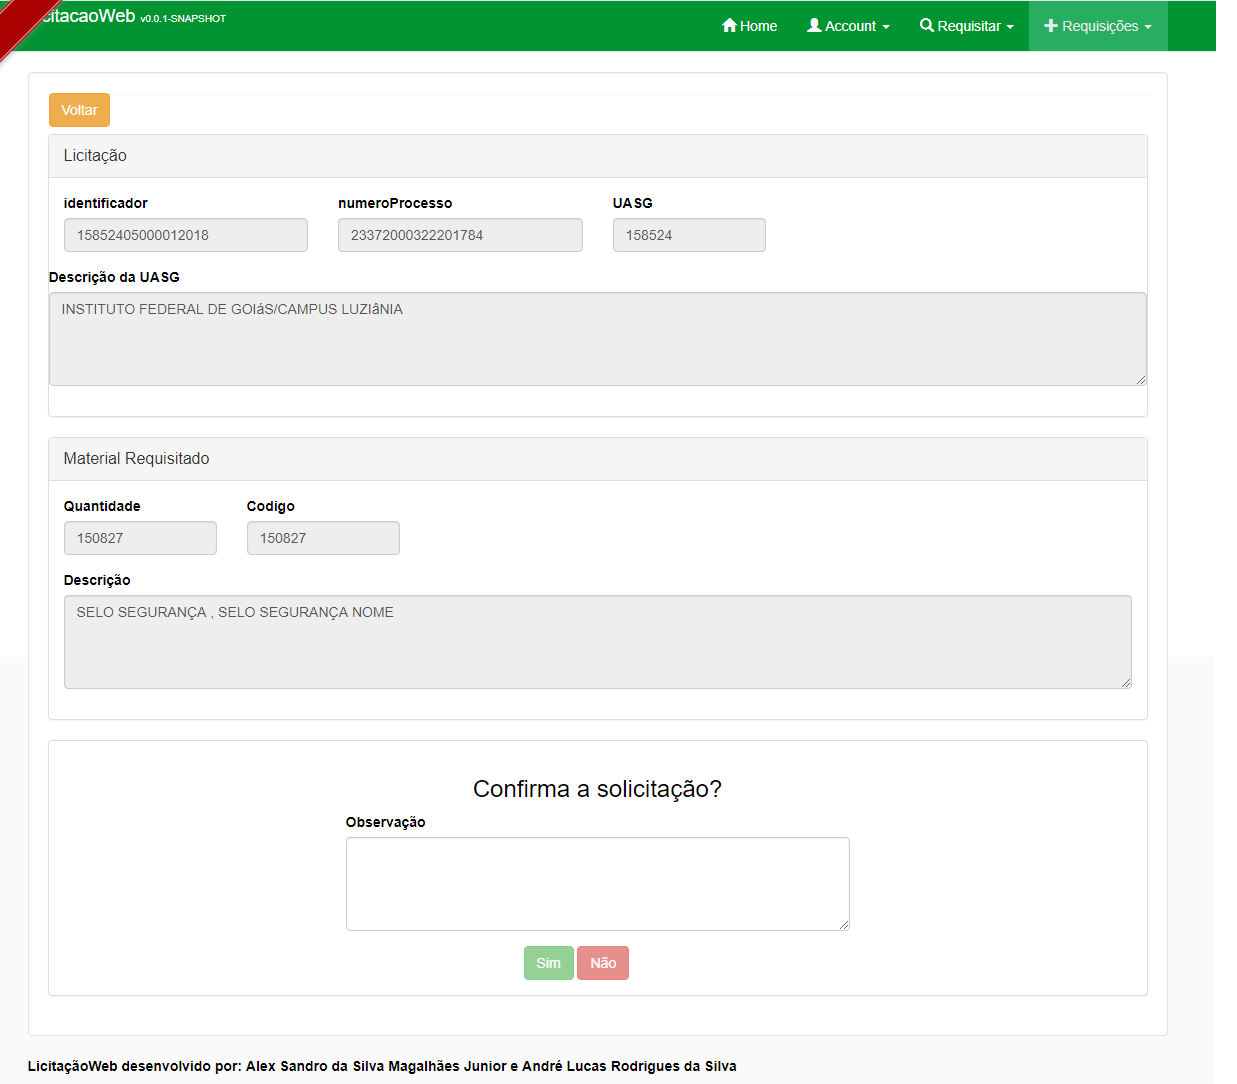
\includegraphics[width=0.95\textwidth]{figuras/prototipo007.png}
    \caption[PROT007: Analisar Requisições]{PROT007: Analisar Requisições.}
    \label{PROT007}
\end{figure}

\begin{figure}[htbp]
    \centering
    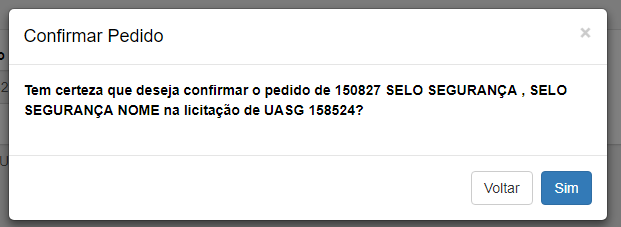
\includegraphics[width=0.95\textwidth]{figuras/prototipo008.png}
    \caption[PROT008: Confirmar Resposta]{PROT008: Confirmar Resposta.}
    \label{PROT008}
\end{figure}

\chapter{Caso de uso 004}\label{CASO004}

\section*{Resposta Requisições}

\subsection*{Descrição}
O sistema permitirá que o usuário veja á resposta do pedido de participação em uma licitação.

\subsection*{Atores}
Servidor público.

\subsection*{Pré-condições}
O Ator deverá estar autenticado e autorizado.

\subsection*{Fluxo Principal}
\begin{enumerate}
    \item Ator aciona o item de menu ``Requisiçõe''~ e o item do submenu ''Resposta''.[\regra{rn014}].
    \item\label{FP004002} Sistema exibe a tela de Resposta de  Requisições~[\prototipo{PROT009}]
    \item\label{FP004003} Ator clica em resposta, irá se aberto uma tela de auxílio com a resposta.~[\regra{rn013}]~[\prototipo{PROT010}].
\end{enumerate}

\subsection*{Fluxo Alternativo}
\begin{enumerate}
    \item Se no Passo~\ref{FP004003} do Fluxo Principal, o ator clicar em ``Voltar'', o sistema retorna à tela anterior~[\prototipo{PROT009}]
\end{enumerate}

\subsection*{Regras de Negócio}

\subsubsection*{RN001}\label{rn014}
O ator deve estar autenticado e autorizado.

\subsubsection*{RN002}\label{rn013}
O botão "Resposta" deve ser habilitado quando a situação estiver como “Aceito” ou "Rejeitado".

\subsection*{Protótipos}
\begin{figure}[htbp]
    \centering
    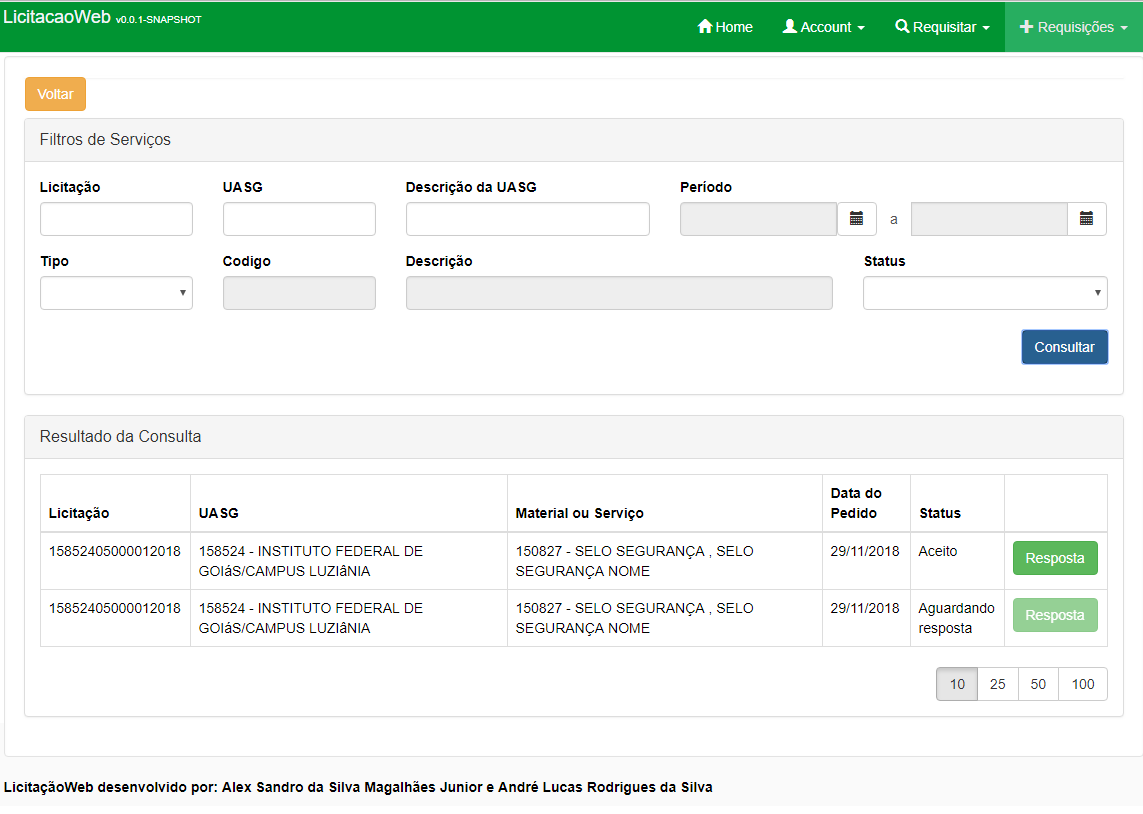
\includegraphics[width=0.95\textwidth]{figuras/prototipo009.png}
    \caption[PROT009: Lista de Requisições]{PROT009: Lista de Requisições.}
    \label{PROT009}
\end{figure}

\begin{figure}[htbp]
    \centering
    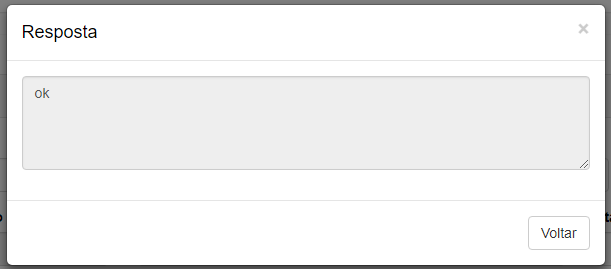
\includegraphics[width=0.95\textwidth]{figuras/prototipo010.png}
    \caption[PROT010: Resposta da Requisição]{PROT010: Resposta da Requisição.}
    \label{PROT010}
\end{figure}

\end{anexosenv}